\section{Simulation of Random Variables}
\label{sec:sim-of-rand-var}

\subsection{Random Number Generators}

Obtaining a good random variable is not a simple task. In the fields sensitive to good random numbers, their generation is typically related to an accurate measurement of some physical variable, for example, the computer time or noise.

More often than not, a \textit{pseudo-random number generator} is utilized. This is nothing but a very \textit{long list of numbers}. A user specifies a \textit{random number seed} that points to the location from which this list will be read. It should be noted that if the same computer code is
executed with the same seed, then the same random numbers get generated, leading to identical results. Often each seed is generated within the system, which of course improves the quality of random numbers.

Instead of a computer, a \textbf{table of random numbers} is often used for small-size studies.

One way or another, a random number generator or a table of random numbers delivers to us Uniform random variables $U_1,\ U_2,\ \ldots \in (0,\ 1)$. The next three subsections show how to transform them into a random variable $X$ with the given desired distribution $F(x)$.

\begin{formula}{NOTATION}
  \begin{center}
    $U;\ U_1,\ U_2,\ \ldots$ = \textnormal{generated Uniform(0, 1) random variables}
  \end{center}
\end{formula}

\subsection{Discrete Methods}

At this point, we have obtained one or several independent Uniform(0,1) random variables by means of a random number generator or a table of random numbers. Variables from certain simple distributions can be immediately generated from this.

\begin{example}{ (Bernoulli)}
  First, simulate a Bernoulli trial with probability of success $p$. For a Standard Uniform variable $U$, define
  \begin{equation*}
    X = \begin{cases}
      1 &\textnormal{if } U < p\\
      0 &\textnormal{if } U \geq p
    \end{cases}
  \end{equation*}
  We call it ``a success'' if $X = 1$ and ``a failure'' if $X = 0$. Using the Uniform distribution of $U$, we find that
  \begin{equation*}
    \prob{\textnormal{ success }} = \prob{U < p} = p
  \end{equation*}
  Thus, we have generated a Bernoulli trial, and $X$ has Bernoulli distribution with the desired probability $p$, see Figure 1a.

  A MATLAB code for this scheme is
  \begin{minted}[]{matlab}
    U = rand;
    X = (U < p)
  \end{minted}
\end{example}

\begin{example}{ (Binomial)}
  Once we know how to generate Bernoulli variables, we can obtain a Binomial variable as a sum of $n$ independent Bernoulli. For this purpose, we start with $n$ Uniform random numbers, for example:
  \begin{minted}[]{matlab}
    n = 20; p = 0.68;
    U = rand(n, 1); % generates an $n \times 1$ 
                    % vector of uniform 
                    % random numbers
    X = sum(U < p)
  \end{minted}
\end{example}

\begin{example}{ (Geometric)}
  A while-loop of Bernoulli trials will generate a Geometric random variable. We run the loop of trials until the first success occurs. Variable $X$ counts the number of failures:
  \begin{minted}[]{matlab}
    X = 1; % Need at least one trial
    while rand > p; % Continue while there
                    % are failures
      X = X+1;
    end; % Stop at the first success
    X
  \end{minted}
\end{example}

\begin{example}{ (Negative Binomial)}
  Just as in Example 2, once we know how to generate a Geometric variable, we can generate a number of them and obtain a Negative Binomial($k$, $p$) variable as a sum of $k$ independent Geometric($p$) variables.
  \begin{minted}{matlab}
    p = 0.16; X = 0; i = 0;
    while i < k;
      G = 1;
      while rand > p;
        G = G+1;
      end;
      X = X+G;
    end;    
  \end{minted}
\end{example}

\begin{figure}[H]
  \centering
  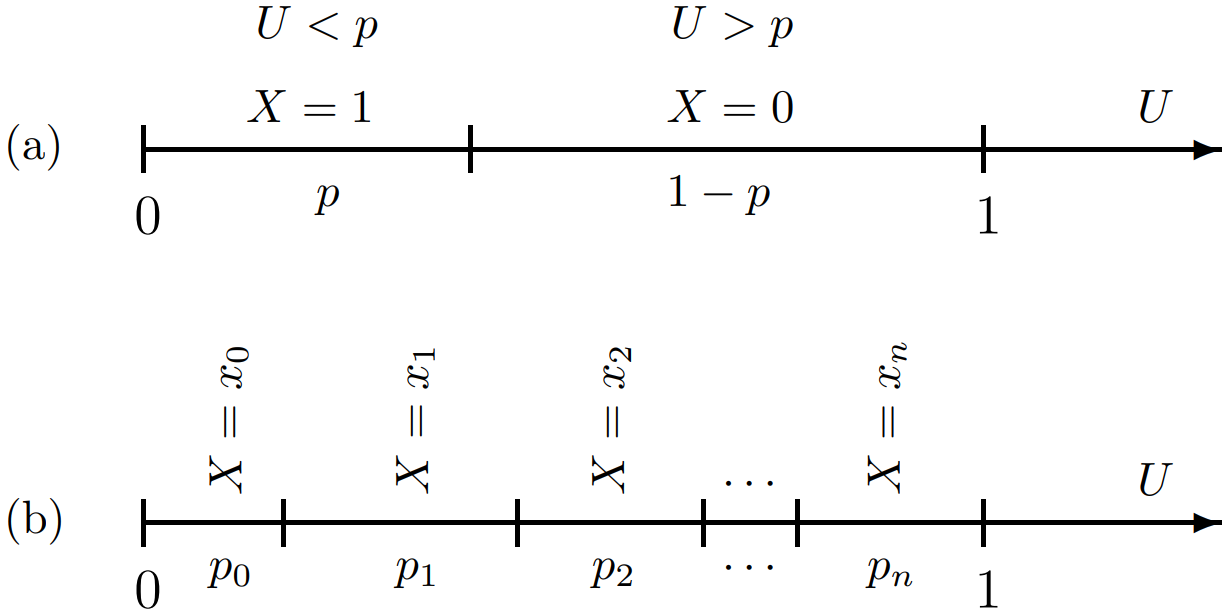
\includegraphics[width=\linewidth]{img/fig-5.2.png}
  \caption{}
\end{figure}

\subsubsection{Arbitrary Discrete Distribution}

Example 1 can be extended to any arbitrary discrete distribution. In this Example, knowing that the random number generator returns a number between 0 and 1, we divided the interval $\left[ 0,\ 1 \right]$ into two parts, $p$ and $(1 - p)$ in length. Then we determined the value of $X$ according to the part where the generated value of $U$ fell, as in Figure 1a.

Now consider an arbitrary discrete random variable $X$ that takes values $x_0$, $x_1$, $\ldots$ with probabilities $p_0$, $p_1$, $\ldots$,
\begin{align*}
  p_i = \prob{X = x_i}, &&\sum_{i=1} p_i = 1
\end{align*}
The scheme similar to Example 1 can be applied as follows.

\vspace*{\fill}
\columnbreak

\paragraph{Algorithm 5.1} (Generating Discrete Variables)
\begin{enumerate}
  \item Divide the interval $\left[ 0,\ 1 \right]$ into subintervals as shown in Figure 1b,
    \begin{align*}
      A_0 &= \left[ 0,\ p_0 \right)\\
      A_1 &= \left[ p_0,\ p_0 + p_1 \right)\\
      A_1 &= \left[ p_0 + p_1,\ p_0 + p_1 + p_2 \right)\\
          &\ \ \textnormal{etc.}
    \end{align*}
    Subinterval $A_i$ will have length $p_i$; there may be a finite or infinite number of them, according to possible values of $X$.
  
  \item Obtain a Standard Uniform random variable from a random number generator or a table of random numbers.
  
  \item If $U$ belongs to $A_i$, let $X = x_i$.  
\end{enumerate}

From the Uniform distribution, it follows again that
\begin{equation*}
  \prob{X = x_i} = \prob{U \in A_i} = p_i
\end{equation*}
Hence, the generated variable $X$ has the desired distribution.

Notice that contrary to Examples 2 and 4, this algorithm is economic as it requires only one Uniform random number for each generated variable.

Values $x_i$ can be written in any order, but they have to correspond to their probabilities $p_i$.

\end{multicols}

\begin{example}{ (Poisson)}
  Let us use Algorithm 5.1 to generate a Poisson variable with parameter $\lambda = 5$. Recall that a Poisson variable takes values $x_0 = 0$, $x_1 = 1$, $x_2 = 2$, $\ldots$ with probabilities
  \begin{equation*}
    p_i = \prob{X = x_i} = e^{-\lambda}\frac{\lambda^{i}}{i!} \textnormal{ for } i =0,1,2,...
  \end{equation*}
  Following the algorithm, we generate a Uniform random number $U$ and find the set $A_i$ containing $U$, so that
  \begin{equation*}
    p_0 + \ldots + p_{i-1} \leq U < p_0 + \ldots + p_{i-1} + p_i
  \end{equation*}
  or, in terms of the cumulative distribution function,
  \begin{equation*}
    F(i - 1) \leq U < F(i)
  \end{equation*}
  This can be done in MATLAB by means of a while-loop:
  \begin{minted}{matlab}
    lambda = 5; % Parameter
    U = rand; % Generated Uniform variable
    i = 0; % Initial value
    F = exp(-lambda); % Initial value, F(0)
    while (U >= F); % The loop ends when U < F(i)
      F = F + exp(-lambda) * lambda^i/gamma(i+1);
      i = i + 1;
    end;
    X=i
  \end{minted}
\end{example}

\begin{multicols}{2}
\setlength{\columnsep}{1.5cm}
\setlength{\columnseprule}{0.2pt}

\subsection{Inverse Transform Method}

As Algorithm 5.1 applies to all discrete distributions, we now turn attention to the generation of continuous random variables. The method will be based on the following simple yet surprising fact.
\begin{theorem}{}
  Let $X$ be a continuous random variable with cdf $F_X(x)$. Define a random variable $U = F_X(X)$. The distribution of $U$ is Uniform(0,1).
\end{theorem}
\begin{proof}
  First, we notice that $0 \leq F(x) \leq 1$ for all $x$, therefore, values of $U$ lie in $\left[ 0,\ 1 \right]$. Second, for any $u \in \left[ 0,\ 1 \right]$, find the cdf of $U$,
  \begin{align*}
    F_U(u) &= \prob{U \leq u}\\
           &= \prob{F_X(X) \leq u}\\
           &= \prob{X \leq F_X^{-1}(u)}\\
           &= F_X(F^{-1}_X(u))\\
           &= u
  \end{align*}
  In the case if $F_X$ is not invertible, let $F^{-1}_X(u)$ denote the smallest $x$ such that $F_X(x) = u$.

  We see that $U$ has cdf $F_U(u) = u$ and density $f_U(u) = F_U'(u) = 1$ for $0 \leq u \leq 1$. This is the Uniform(0, 1) density, hence, $U$ has Uniform(0, 1) distribution.
\end{proof}

Regardless of the initial distribution of $X$, it becomes Uniform(0,1), once $X$ is substituted into its own cumulative distribution function!

\subsubsection{Arbitrary Continuous Distribution}

In order to generate variable $X$ with the given continuous cdf $F$, let us revert the formula $U = F(X)$. Then $X$ can be obtained from a generated Standard Uniform variable $U$ as $X = F^{-1}(U)$.

\paragraph{Algorithm 5.2} (Generating Continues Variables)
\begin{enumerate}
  \item Obtain a Standard Uniform random variable from a random number generator.
  \item  Compute $X = F^{-1}(U)$. In other words, solve the equation $F(X) = U$ for $X$.
\end{enumerate}

\vspace*{\fill}
\columnbreak

\begin{example}{ (Exponential)}
  How shall we generate an Exponential variable with parameter $\lambda$? According to Algorithm 5.2, we start by generating a Uniform random variable $U$. Then we recall that the Exponential cdf is $F(x) = 1 - e^{-\lambda x}$ and solve the equation
  \begin{equation*}
    1 - e^{-\lambda x} = U
  \end{equation*}
  The result is
  \begin{equation}
    X = - \frac{1}{\lambda} \ln(1-U)
  \end{equation}
  Can this formula be simplified? By any rule of algebra, the answer is ``no''. On the other hand, $(1 - U)$ has the same distribution as $U$, Standard Uniform. Therefore, we can replace $U$ by $(1 - U)$, and variable
  \begin{equation}
    X_1 = - \frac{1}{\lambda} \ln(U)
  \end{equation}
  although different from $X$, will also have the desired Exponential($\lambda$) distribution.
\end{example}

\begin{example}{ (Gamma)}
  Gamma cdf has a complicated integral form, not mentioning $F^{-1}$, needed for Algorithm 5.2. There are numerical methods of solving the equation $F(X) = U$, but alternatively, much simpler, for any integer $\alpha$, a Gamma variable can be generated as a sum of $\alpha$ independent Exponential variables:
  \begin{minted}{matlab}
    X = sum( -1/lambda * log(rand(alpha,1)) )    
  \end{minted}
\end{example}

\subsubsection{Discrete Distributions Revisited}

Algorithm 5.2 is not directly applicable to discrete distributions because the inverse function $F^{-1}$ does not exist in the discrete case. In other words, the key equation $F(X) = U$ may have either \textit{infinitely many roots} or \textit{no roots} at all.

Moreover, a discrete variable $X$ has a finite or countable range of possible values, and so does $F(X)$. The probability that $U$ coincidentally equals one of these values is $0$. We conclude that the equation $F(X) = U$ has \textit{no roots} with probability $1$.

Let us modify the scheme in order to accommodate discrete variables. Instead of solving $F(x) = U$ exactly, which is impossible, we solve it approximately by finding $x$, the smallest possible value of $X$ such that $F(x) > U$.

The resulting algorithm is described below.

\vspace*{\fill}
\columnbreak

\paragraph{Algorithm 5.3} (Generating Discrete Variables, Revisited)
\begin{enumerate}
  \item Obtain a Standard Uniform random variable from a random number generator or a table of random numbers.
  \item Compute $X = \min \{ x \in S \textnormal{ such that } F(x) > U \}$, where $S$ is a set of possible values of $X$.  
\end{enumerate}
Algorithms 5.1 and 5.3 are equivalent if values $x_i$ are arranged in their increasing order in Algorithm 5.1.

\begin{example}{ (Geometric revisited)}
  Applying Algorithm 5.3 to Geometric cdf
  \begin{equation*}
    F(x) = 1 - (1 - p)^x
  \end{equation*}
  we need to find the smallest integer $x$ satisfying the inequality (solve it for $x$)
  \begin{equation*}
    x > \frac{\ln(1 - U)}{\ln(1 - p)}
  \end{equation*}v
  The smallest such integer is the ceiling
  \begin{equation}
    X = \left\lceil \frac{\ln(1 - U)}{\ln(1 - p)} \right\rceil
  \end{equation}
\end{example}

\subsubsection{Exponential-Geometric Relation}

The formula (5.3) appears very similar to (5.1). With $\lambda = - \ln(1 - p)$, our generated Geometric variable is just the ceiling of an Exponential variable! In other words, the ceiling of an Exponential variable has Geometric distribution.

This is not a coincidence.
\begin{itemize}
  \item Exponential is the continuous analogue of geometric
  \item Both have the memoryless property.
\end{itemize}